\documentclass[10.5pt]{article}
\usepackage[margin=0.85in]{geometry}
\usepackage{xcolor,amsmath,amssymb,graphicx,booktabs,enumitem,hyperref,titlesec,tikz,tabularx,array,caption,float}
\usepackage[most]{tcolorbox}
\usetikzlibrary{arrows.meta,positioning}
\hypersetup{colorlinks=true,urlcolor=blue!60!black,linkcolor=black}
\titlespacing*{\section}{0pt}{9pt}{3pt}
\titlespacing*{\subsection}{0pt}{6pt}{2pt}
\titleformat{\section}{\large\bfseries}{\thesection.}{0.4em}{}
\titleformat{\subsection}{\normalsize\bfseries}{\thesubsection}{0.4em}{}
\setlist{nosep,leftmargin=1.3em,topsep=2pt}
\setlength{\parskip}{4pt}\setlength{\parindent}{0pt}
\captionsetup{font=small,labelfont=bf}
\newcommand{\todo}[1]{\textcolor{red!70!black}{#1}}
\newtcolorbox{plain}[1]{colback=blue!3,colframe=blue!40!black,boxrule=0.5pt,arc=2pt,
  left=5pt,right=5pt,top=3pt,bottom=3pt,fonttitle=\bfseries\small,title={#1}}
\newtcolorbox{mathbox}[1]{colback=gray!4,colframe=gray!50,boxrule=0.5pt,arc=2pt,
  left=5pt,right=5pt,top=3pt,bottom=3pt,fonttitle=\bfseries\small,coltitle=black,title={#1}}

\begin{document}
\begin{center}
{\Large\bfseries Progress Report 1}\\[3pt]
{\large Multiscale Modeling and Visualization of Drug Absorption, Distribution and Vascular Transport}\\[4pt]
02-601 Programming for Scientists \quad$\cdot$\quad Team \todo{[Team name]}\\
\todo{[Person 1], [Person 2], [Person 3], [Person 4]}\\[3pt]
\textbf{Code (work in progress):} \todo{\url{https://github.com/[username]/drug-diffusion-project}}
\end{center}

\begin{plain}{Summary in three sentences}
We are building a computer simulation that follows a medicine from the moment it is swallowed (or injected)
until it has been removed from the body, and that also shows how the drug moves inside one small blood vessel.
For this first checkpoint, every core part of the program works: the whole-body model, the blood-vessel model,
the link between them, pictures and movies, a first interactive app, and 22 automatic tests that check the results.
The rest of the semester goes into better input data, more drugs, the interactive app, and documentation.
\end{plain}

%==========================================================================
\section{The question we are asking}
When you take a painkiller, it does not act instantly. The pill dissolves in the stomach, moves into the
intestine, passes into the blood, goes through the liver (which destroys part of it), spreads through the
body, and is slowly removed by the liver and kidneys. Doctors care about \emph{how high} the drug level in
the blood gets, \emph{how soon}, and \emph{for how long}, because these decide whether a drug works and whether
it is safe. Eating a meal before taking the pill can change all three.

Our project answers two linked questions with a computer:
\begin{enumerate}
\item \textbf{Whole body (hours):} after a dose, how much drug is in the stomach, intestine, liver, blood
and the rest of the body at every moment, and how does a meal change this?
\item \textbf{One blood vessel (seconds):} at a chosen moment, how is the drug actually spread out
\emph{inside} a small blood vessel as the blood carries it along?
\end{enumerate}

%==========================================================================
\section{The big idea: two zoom levels}
Simulating every blood vessel in the body is impossible on a laptop. We therefore use the same trick as a map
app: a \textbf{zoomed-out view} of the whole body that only tracks \emph{how much} drug is in each organ, and a
\textbf{zoomed-in view} of a single small vessel that tracks \emph{where} the drug is. The zoomed-out model produces
the drug level in the blood over time. We then hand that number to the zoomed-in model as the concentration of
the blood flowing into the vessel. This hand-over is the \emph{link} (``coupling'') between the two models.

\begin{figure}[H]
\centering
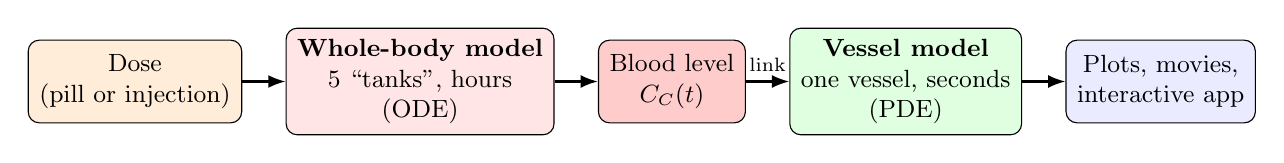
\begin{tikzpicture}[node distance=0.55cm,
  box/.style={draw,rounded corners,align=center,minimum height=1.05cm,font=\small,inner sep=4pt},
  arr/.style={-{Latex[length=2.2mm]},thick}]
\node[box,fill=orange!15] (dose) {Dose\\(pill or injection)};
\node[box,fill=red!10,right=of dose] (ode) {\textbf{Whole-body model}\\5 ``tanks'', hours\\(ODE)};
\node[box,fill=red!20,right=of ode] (cc) {Blood level\\$C_C(t)$};
\node[box,fill=green!12,right=of cc] (pde) {\textbf{Vessel model}\\one vessel, seconds\\(PDE)};
\node[box,fill=blue!8,right=of pde] (viz) {Plots, movies,\\interactive app};
\draw[arr] (dose)--(ode); \draw[arr] (ode)--(cc); \draw[arr] (cc)--node[above,font=\scriptsize]{link}(pde); \draw[arr] (pde)--(viz);
\end{tikzpicture}
\caption{The pipeline. The output of the whole-body model (blood concentration over time) becomes the input of the
vessel model. Information flows in one direction only in the core project.}
\end{figure}

%==========================================================================
\section{Part 1 -- The whole-body model}
\subsection{The body as five connected water tanks}
Imagine five tanks connected by pipes. Each tank holds a certain amount of drug, and drug flows through the pipes
from one tank to the next. We assume each tank is \emph{well mixed} (like stirred soup), so one number per tank is
enough: ``how many milligrams of drug are in it right now''.

\begin{center}\small
\begin{tabularx}{\linewidth}{@{}l X@{}}
\toprule
\textbf{Tank} & \textbf{What happens there (in everyday words)}\\\midrule
1. Stomach & The swallowed pill starts here. The stomach empties its contents into the intestine bit by bit.\\
2. Intestine & The drug is absorbed through the gut wall into the blood that goes to the liver.\\
3. Liver & The liver is the body's chemical cleaning plant. It destroys part of the drug \emph{before} it reaches
the rest of the body (the ``first-pass effect'') and keeps cleaning the blood afterwards.\\
4. Central blood & All circulating blood, treated as one big mixed pool. This is the drug level a blood test
would measure, and the number that matters most.\\
5. Peripheral tissue & Muscle, fat, skin and so on, lumped together. Drug moves in when the blood level is high and
moves back out later, like a sponge that soaks up and then releases water.\\
Kidneys & Not a tank, but a drain on the blood tank that removes drug into the urine.\\
\bottomrule
\end{tabularx}
\end{center}

\subsection{The rule behind every equation: change = in -- out}
For each tank we write one simple balance: \emph{how fast the amount changes = what flows in -- what flows out.}
Mathematicians call this kind of equation an \textbf{ordinary differential equation (ODE)}. For example, the stomach
only empties, at a rate proportional to what it still holds. With $k_{GE}=4$ per hour, about half of the stomach
content leaves in the first 10 minutes when fasted. A meal slows this to $k_{GE}=1$ per hour (half after about
40 minutes). The full set of equations, which our code implements line by line, is:

\begin{mathbox}{The five equations ($A$ = amount in mg, $C=A/V$ = concentration, $t$ in hours)}
\small
\begin{align*}
\text{stomach:}\quad& \tfrac{dA_S}{dt}=-k_{GE}A_S &&\text{empties into the intestine}\\
\text{intestine:}\quad& \tfrac{dA_I}{dt}=k_{GE}A_S-k_aA_I &&\text{in from stomach, out by absorption}\\
\text{liver:}\quad& \tfrac{dA_L}{dt}=F_gk_aA_I+Q_H\big(C_C-\tfrac{C_L}{K_L}\big)-CL_H\tfrac{C_L}{K_L} &&\text{absorbed + exchange -- destroyed}\\
\text{blood:}\quad& \tfrac{dA_C}{dt}=Q_H\big(\tfrac{C_L}{K_L}-C_C\big)-Q_P\big(C_C-\tfrac{C_P}{K_P}\big)-CL_RC_C &&\text{exchange -- removed by kidneys}\\
\text{tissue:}\quad& \tfrac{dA_P}{dt}=Q_P\big(C_C-\tfrac{C_P}{K_P}\big) &&\text{soaks up / releases drug}
\end{align*}
{\footnotesize $k_{GE}, k_a$: emptying and absorption speeds; $Q_H, Q_P$: litres of blood flowing through the liver /
tissue per hour; $CL_H, CL_R$: ``clearance'', the litres of blood the liver / kidneys clean completely per hour;
$K_L, K_P$: how strongly an organ holds on to the drug compared with blood; $F_g$: fraction surviving the gut wall.
Swallowed pill: all of the dose starts in the stomach. Injection (IV): all of it starts in the blood.}
\end{mathbox}

A computer cannot solve these equations ``in one go''. Instead it takes thousands of tiny time steps: from the
current amounts it computes the flows, moves a little drug along every pipe, and repeats. We use the standard
scientific library \texttt{scipy} for this stepping. We also keep three ``counters'' for drug that has left the body
(liver, kidneys, gut), so we can check at every moment that \emph{drug in the body + drug removed = dose}.
Our program satisfies this to 12 decimal places.

\subsection{First results: what the model predicts}
We tested the model with a common painkiller, \textbf{acetaminophen} (Tylenol), 1000\,mg taken by mouth, using
values for a typical 70-kg adult.

\begin{figure}[tbp]
\centering
\includegraphics[width=0.49\linewidth]{../docs/figures/pk_compartments.png}\hfill
\includegraphics[width=0.49\linewidth]{../docs/figures/fed_vs_fasted_curve.png}
\caption{\textbf{Left:} where the 1000\,mg dose is over 12 hours. The stomach (orange) empties within about an hour,
the intestine (brown) briefly fills and empties, much of the drug temporarily sits in body tissue (green), and the
dashed line shows the drug that has been removed. After 12 hours almost all of it has been removed.
\textbf{Right:} blood level on an empty stomach (blue) versus after a meal (orange dashed).}
\end{figure}

To compare curves, pharmacologists use three standard numbers, which our code computes automatically:
\begin{itemize}
\item \textbf{$C_{\max}$} -- the highest blood level reached (``how strong is the peak?'').
\item \textbf{$T_{\max}$} -- when that peak happens (``how quickly does it kick in?'').
\item \textbf{AUC} (area under the curve) -- the total exposure over time (``how much drug did the body see in total?'').
\end{itemize}

\begin{center}\small
\begin{tabular}{lccc}\toprule
Acetaminophen 1000\,mg by mouth & $C_{\max}$ (mg/L) & $T_{\max}$ (hours) & AUC (mg$\cdot$h/L)\\\midrule
Empty stomach (fasted) & 9.3 & 0.9 & 36.3\\
After a meal (fed) & 7.0 & 2.0 & 35.9\\\bottomrule
\end{tabular}
\end{center}

\textbf{How to read this:} after a meal the peak comes about an hour later and is about 25\,\% lower, but the
total exposure (AUC) is almost the same. Food slows the drug down but does not reduce how much of it eventually gets in.
This pattern matches what is generally reported for acetaminophen. The model also predicts that the liver destroys
about 22\,\% of the swallowed dose on its first pass, and that the blood level halves every 2.0 hours. Both are in the
range reported in the pharmacology literature (Forrest et al.\ 1982). These are qualitative checks only. A careful
comparison with published data is planned (Section~8).

%==========================================================================
\section{Part 2 -- Zooming into one blood vessel}
\subsection{What moves the drug inside a vessel}
We now look at one small vessel, 0.2\,mm wide (about two human hairs) and 10\,mm long. Two effects move the drug:
\begin{enumerate}
\item \textbf{Being carried by the flow (``advection'').} Like a leaf on a river, the drug travels with the
blood. Blood does \emph{not} move at one speed: it is fastest in the middle of the vessel and almost still at
the wall, because the wall slows it down by friction. The speed profile is a smooth arch (a parabola), so drug in
the centre races ahead and the incoming drug front looks like a stretched bullet.
\item \textbf{Spreading out (``diffusion'').} Molecules constantly jiggle randomly, so drug slowly spreads from
crowded places to empty ones, like a drop of ink in still water. How fast it spreads depends on the size of the molecule
and the ``thickness'' of the liquid. We calculate this from the molecule's weight with a standard physics formula
(Stokes--Einstein) instead of guessing it.
\end{enumerate}
In our vessel the flow is about 400 times stronger than sideways spreading. Drug crosses the 10\,mm vessel in
about 3--5 seconds, but would need about 20 seconds to spread from the centre to the wall by diffusion alone.

\begin{mathbox}{The vessel equation (a ``partial differential equation'', PDE)}
\vspace{-4pt}
\[
\underbrace{\frac{\partial c}{\partial t}}_{\text{change over time}}
+\underbrace{u(y)\,\frac{\partial c}{\partial x}}_{\text{carried by the flow}}
=\underbrace{D\Big(\frac{\partial^2 c}{\partial x^2}+\frac{\partial^2 c}{\partial y^2}\Big)}_{\text{spreading by diffusion}},
\qquad u(y)=2\bar u\Big(1-\frac{y^2}{R^2}\Big)
\]
{\footnotesize $c(x,y,t)$: drug concentration at position $x$ (along the vessel) and $y$ (across it) at time $t$;
$\bar u=2$\,mm/s: average blood speed; $R$: vessel radius; $D$: diffusion coefficient. It is called \emph{partial}
because the concentration now depends on position \emph{and} time, unlike the tanks of Part~1.}
\end{mathbox}

\subsection{How the computer solves it}
We cut the vessel into a grid of $200\times24$ small rectangles (``cells''), like a spreadsheet in which each cell
stores the drug concentration in that little region. Every 5 milliseconds of simulated time, the program works out how
much drug crosses each cell border, carried by the flow or by diffusion, and updates every cell. Whatever leaves one
cell enters its neighbour, so no drug is accidentally created or lost (this approach is called the \emph{finite-volume
method}). Two technical details keep the result trustworthy:
\begin{itemize}
\item \textbf{Time step limit.} If the time step were too large, drug would ``jump over'' cells and the numbers would
explode. The program automatically picks a safe step size (the CFL condition).
\item \textbf{No fake ripples.} A simple method smears the sharp drug front, and a naive accurate method creates
unphysical wiggles. We use a standard compromise (a ``flux limiter'') that keeps fronts sharp without wiggles.
\end{itemize}

\subsection{The link between the two models}
At the vessel entrance we set the drug concentration equal to the blood level that the whole-body model predicts at
the chosen moment:
\[
\text{concentration entering the vessel} \;=\; C_C(\text{chosen body time}).
\]
Figure~3 shows this link. The left panel is the whole-body blood curve. We pick three moments: \textbf{A} (15 minutes,
drug still being absorbed), \textbf{B} (1 hour, near the peak) and \textbf{C} (6 hours, drug being removed). For each
moment we run the vessel model, and the right panels show the vessel 5 seconds after the drug starts flowing in.
Darker green means more drug. The same vessel looks very different depending on \emph{when} in the body's timeline we
look, which is exactly what the two-level design is meant to show.

\begin{figure}[tbp]
\centering
\includegraphics[width=0.82\linewidth]{../docs/figures/multiscale_coupling.png}
\caption{The two models connected. \textbf{Left:} blood level after a 1000\,mg acetaminophen tablet (empty stomach),
from the whole-body model. \textbf{Right:} the small vessel at moments A, B and C. The inflowing blood carries
exactly the blood level read off the left curve. The lighter region at the right end of each vessel is blood that the
drug has not reached yet. It arrives first along the fast-flowing centre line.}
\end{figure}

%==========================================================================
\section{How we know the program is correct}
A simulation is only useful if we can trust it, so we wrote 22 automatic tests that run in about 2 seconds
(\texttt{python -m unittest}). Each test compares the program with something we know must be true:

\begin{center}\small
\begin{tabularx}{\linewidth}{@{}>{\raggedright}p{0.33\linewidth} X@{}}
\toprule
\textbf{Test} & \textbf{Why it matters}\\\midrule
Drug is never created or lost (both models) & The most basic law: total drug = dose. Errors are below $10^{-12}$.\\
No absorption $\Rightarrow$ nothing reaches the blood & If the gut absorbs nothing, the blood level must stay at zero.\\
No liver/kidney cleaning $\Rightarrow$ nothing is removed & Switching off removal must keep all drug in the body.\\
Injection acts immediately, a pill is delayed & An injection goes straight into the blood, a pill must be absorbed first.\\
Simple cases match textbook formulas & With only one tank, the program reproduces the known exact answer, and long-run
exposure matches the classic formula AUC = (fraction absorbed $\times$ dose) / clearance.\\
Pure spreading matches the exact solution & With the flow switched off, drug spreads exactly as physics predicts.\\
Finer grid gives the same answer & Results change by less than 2\,\% when the grid is made twice as fine, so the grid
is not distorting the answer.\\
No negative or overshooting values & Concentrations never go below zero or above the incoming level.\\
The link works & The concentration entering the vessel equals the whole-body blood level at the chosen time.\\
\bottomrule
\end{tabularx}
\end{center}

%==========================================================================
\section{How the code is organised}
The program is written in Python using object-oriented design: each \emph{class} is a self-contained building
block with one job, and the blocks connect through agreed ``contracts'' (inputs and outputs). This lets the four of
us work in parallel without breaking each other's code. Every function has a description, and the code is commented
in plain language.

\begin{center}\small
\begin{tabularx}{\linewidth}{@{}l l X@{}}
\toprule
\textbf{Building block} & \textbf{File} & \textbf{Job}\\\midrule
\texttt{Drug}, \texttt{Physiology}, \texttt{Scenario} & \texttt{drug.py}, \texttt{physiology.py} & Hold the input numbers: the medicine, the person, and the situation (pill/injection, fed/fasted).\\
\texttt{PKModel}, \texttt{PKResult} & \texttt{pk\_model.py} & The five-tank whole-body model and its results.\\
\texttt{PKMetrics} & \texttt{metrics.py} & Computes $C_{\max}$, $T_{\max}$, AUC and half-life.\\
\texttt{VesselModel}, \texttt{VesselResult} & \texttt{vessel.py} & The blood-vessel model and its results.\\
\texttt{Simulation} & \texttt{simulation.py} & Connects the two models (the ``link'').\\
\texttt{Visualizer}, \texttt{app.py} & \texttt{visualization.py} & Graphs, movies and the interactive app.\\
\bottomrule
\end{tabularx}
\end{center}
All input numbers live in separate data files (\texttt{drugs.json}, \texttt{physiology.json}), and the source of
every number is listed in \texttt{references.csv}. Two drugs are included so far: acetaminophen and caffeine.

%==========================================================================
\section{What we plan to do next}
\begin{itemize}
\item \textbf{By checkpoint 2 (Nov 9):} check every input number against original scientific sources and add one or
two more drugs with published fed/fasted data; compare our $C_{\max}$, $T_{\max}$ and AUC with published measurements;
run a careful accuracy study of the vessel model.
\item \textbf{By the final deadline (Dec 11):} finish the interactive app (choose a drug, dose, pill or injection, meal or
no meal, then move a time slider and watch the vessel); add the vessel movie and a ``glowing body'' view; write the
documentation web page with example results; prepare the presentation.
\item \textbf{Extras, only if time allows:} a leaky vessel wall that lets drug pass into surrounding tissue (we already
have a working prototype, switched off by default); feedback from the vessel back to the whole body; a separate kidney
compartment; a beating (pulsing) blood flow.
\end{itemize}

%==========================================================================
\section{Problems we are running into}
\begin{itemize}
\item \textbf{Finding the right input numbers.} Scientific papers usually report summary values (for example how quickly
the whole body removes a drug), not the exact numbers our tanks need (for example how strongly the liver alone
removes it). We currently work them out from the summary values with standard formulas and record every step in
\texttt{references.csv}. Data on how meals affect a particular drug are scattered and sometimes contradictory.
\item \textbf{Very different time scales.} The body model runs over hours, the vessel model over seconds. During a
10-second vessel run, the body's blood level barely changes, so the vessel picture mainly shows how fresh drug
washes in and fills the vessel. We need to explain clearly what the vessel view adds (where the drug is and how fast
it gets there) and what it cannot show unless we add the leaky wall.
\item \textbf{Computing time.} The vessel model needs about 2000 small time steps for 10 seconds of blood flow. That
is fine for figures, but it may feel slow in the interactive app. We will save results that were already computed
and use a coarser preview grid.
\item \textbf{Flat picture of a round vessel.} Our vessel is a flat 2-D slice through a round tube. Sideways spreading
in a real tube behaves slightly differently, and we plan to measure how large this difference is.
\end{itemize}

%==========================================================================
\section{Who did what}
\begin{itemize}
\item \todo{[Person 1]} -- \textbf{Whole-body model:} the five-tank equations, pill and injection starting conditions,
mass-balance and special-case tests.
\item \todo{[Person 2]} -- \textbf{Vessel model:} grid, blood-flow profile, flow-and-spreading calculation,
time-step safety analysis, vessel tests.
\item \todo{[Person 3]} -- \textbf{Input data and checks:} drug, body and fed/fasted parameters, data files and
source list, $C_{\max}$/$T_{\max}$/AUC calculation and tests.
\item \todo{[Person 4]} -- \textbf{Linking and visuals:} the \texttt{Simulation} class that connects the models,
all figures and movies, the first interactive app, README and this report.
\end{itemize}
\textbf{Use of AI tools.} As allowed by the course policy, the first draft of the checkpoint-1 code was written with an AI
assistant (Claude), following our own technical design document. Every file names its author and a human reviewer.
Each team member has reviewed, run and tested the module they own and can explain it. The remaining work will be written
by the team so that AI-written code stays under the 50\,\% limit.

%==========================================================================
\section*{Glossary}
{\small
\begin{tabularx}{\linewidth}{@{}l X@{}}
\textbf{Pharmacokinetics (PK)} & The study of how the body absorbs, distributes and removes a drug.\\
\textbf{Compartment} & A part of the body treated as one well-mixed tank (e.g. ``the liver'').\\
\textbf{Concentration} & Amount of drug per volume of liquid, here in milligrams per litre (mg/L).\\
\textbf{Clearance} & How many litres of blood an organ cleans completely of drug per hour.\\
\textbf{First-pass effect} & The part of a swallowed drug destroyed by the liver before it reaches the rest of the body.\\
\textbf{ODE / PDE} & Equations describing how things change. In an ODE quantities change only over time; in a PDE they
change over time \emph{and} position.\\
\textbf{Advection / diffusion} & Being carried by the flow / spreading out by random molecular motion.\\
\textbf{Finite-volume method} & Solving a PDE by dividing space into small cells and tracking what moves between them.\\
\textbf{IV} & Intravenous: injected directly into a vein.\\
\end{tabularx}}

\vspace{4pt}
{\footnotesize\textbf{References.} Forrest JA, Clements JA, Prescott LF (1982), Clinical pharmacokinetics of paracetamol,
\textit{Clin.\ Pharmacokinet.} 7:93--107. Arnaud MJ (2011), Pharmacokinetics and metabolism of natural methylxanthines,
\textit{Handb.\ Exp.\ Pharmacol.} 200:33--91. Davies B, Morris T (1993), Physiological parameters in laboratory animals and
humans, \textit{Pharm.\ Res.} 10:1093--1095. Brown RP et al.\ (1997), Physiological parameter values for PBPK models,
\textit{Toxicol.\ Ind.\ Health} 13:407--484. LeVeque RJ (2002), \textit{Finite Volume Methods for Hyperbolic Problems},
Cambridge University Press.}
\end{document}
